% 1 Page Parameters
% 2 Special Commands for Editions
% 3 Content Modifications
% 4 Counters and Parameters
% 5 Section Coloring
% 6 Utilities
% 7 
% 8 Figures and Captions
% 9 Examples and Exercises
% 10 Special Boxes

%\renewcommand\chapter{\if@openright\cleardoublepage\else\clearpage\fi
%                    \thispagestyle{fancy}%
%                    \global\@topnum\z@
%                    \@afterindentfalse
%                    \secdef\@chapter\@schapter}
\fancypagestyle{plain}{%
\fancyhf{} % clear all header and footer fields
\fancyhead[RO,RE]{\thepage} %RO=right odd, RE=right even
\renewcommand{\headrulewidth}{0pt}
\renewcommand{\footrulewidth}{0pt}}
\raggedbottom


\newcommand{\stdspace}[0]{3mm}
\newcommand{\stdvspace}[0]{\vspace{\stdspace{}}}
\newcommand{\stdaddvspace}[0]{\addvspace{\stdspace{}}}




%-------------------------------------------------------------
% 1 Page Parameters
% 1.1
\setlength\paperheight{11in}
\setlength\paperwidth{8.5in}
\newcommand{\officialtextheight}{9.7in}
\newcommand{\officialtextwidth}{6in}
%\setlength\paperheight{10in}
%\setlength\paperwidth{8in}
%\newcommand{\officialtextheight}{8.7in}
%\newcommand{\officialtextwidth}{6in}
\newcommand{\officialvoffset}{-0.6in}
\setlength\textheight{\officialtextheight}
\setlength\textwidth{\officialtextwidth}
\setlength\voffset{\officialvoffset}
\renewcommand{\baselinestretch}{1.0}
% 1.2 Margin Size
% 1.2.1 Slim
%\setlength\hoffset{0.25in}
%\setlength\oddsidemargin{0.25in}
%\setlength\evensidemargin{0in}
% 1.2.2 Medium
\setlength\hoffset{3.7mm}
\setlength\oddsidemargin{3mm}
\setlength\evensidemargin{3mm}
% 1.2.3 Wide
%\setlength\hoffset{-5mm}
%\setlength\oddsidemargin{0.5in}
%\setlength\evensidemargin{0.5in}
% 1.3 PDF Parameters
%\setlength\paperheight{11in}
%\setlength\textheight{8.25in}
%\setlength\paperwidth{8.5in}
%\setlength\textwidth{5.45in}
%\setlength\voffset{-10mm}
%\setlength\oddsidemargin{0.75in}
%\setlength\evensidemargin{0.75in}
% 1.4 Margin Spacing
\setlength{\marginparsep}{5mm}
\setlength{\marginparwidth}{20mm}
% 1.5 Page Header
\pagestyle{fancy}
\renewcommand{\headrulewidth}{0pt}
\fancyhead[RO,LE]{\thepage}
\fancyhead[RE]{\leftmark}
\fancyhead[LO]{\rightmark}
\fancyfoot[c]{}
\fancyheadoffset[RO,LE]{0.9in}



% Tablet Version
%\setlength\paperheight{8.82in}\setlength\textheight{8.25in}\setlength\paperwidth{5.7in}\setlength\textwidth{5.45in}\setlength\voffset{-23.5mm}\setlength\hoffset{-27mm}\setlength\oddsidemargin{5mm}\setlength\evensidemargin{5mm}\setlength{\marginparsep}{5mm}\setlength{\marginparwidth}{35mm}\fancyheadoffset[RO,LE]{0.2in}




%-------------------------------------------------------------
% 2 Special Commands for Editions
\newcommand{\referrer}{os4_pdf}
\newcommand{\vspaceB}[1]{}
\newcommand{\hspaceB}[1]{}
\newcommand{\textB}[1]{}
\newcommand{\textC}[1]{}
\newcommand{\D}[1]{#1}



%-------------------------------------------------------------
% 3 Content Modifications
\newcommand{\APVersion}[2]{#2}
\newcommand{\MultipleRegression}[2]{#1}
\newcommand{\MultipleRegressionChapter}[2]{#1}
\newcommand{\SimulationAndRandomization}[1]{#1}
\newcommand{\ANOVASection}[2]{#1}
\newcommand{\GLMSection}[2]{#1}




%-------------------------------------------------------------
% 4 Counters and Parameters
% 4.1 Counters
\newcounter{alwaysOne}
\setcounter{alwaysOne}{1}
\newcounter{alwaysTwo}
\setcounter{alwaysTwo}{2}
\newcounter{alwaysThree}
\setcounter{alwaysThree}{3}
\newcounter{alwaysFour}
\setcounter{alwaysFour}{4}
\newcounter{withinChNum}[chapter]
\setcounter{withinChNum}{0}
\newcounter{eoce}[chapter]
\renewcommand{\theeoce}
    {\arabic{chapter}.\arabic{eoce}}
\newcounter{eocesolch}
\setcounter{eocesolch}{0}
\newcounter{eocesol}[eocesolch]
\renewcommand{\theeocesol}
     {\arabic{eocesolch}.\arabic{eocesol}}
\newcounter{eoceNeedSolution}[chapter]
\renewcommand{\theeoceNeedSolution}
    {\arabic{chapter}.\arabic{eoceNeedSolution}}
\newcounter{eoceReplace}[chapter]
\renewcommand{\theeoceReplace}
    {\arabic{chapter}.\arabic{eoceReplace}}
\newcounter{eoceFF}[chapter]
\renewcommand{\theeoceFF}
    {\arabic{chapter}.\arabic{eoceFF}}
% 4.2 Parameters
\newlength{\exampleAboveBar}
\newlength{\exampleBelowBar}
\setlength{\exampleAboveBar}{-3.15mm}
\setlength{\exampleBelowBar}{-1.15mm}
\newlength{\nexampleAboveBar}
\newlength{\nexampleBelowBar}
\setlength{\nexampleAboveBar}{-1mm}
\setlength{\nexampleBelowBar}{-1mm}
% 4.3 Chapter Declarations
\newcommand\includechapter[2]{
  \setcounter{chapter}{#1}
  \addtocounter{chapter}{-1}
  \normalsize
  \include{#2/TeX/#2}
  \newpage\reviewexercisesheader{}

% 1

\eoce{\qt{Infant mortality\label{infant_mortality}} The infant mortality rate is defined as 
the number of infant deaths per 1,000 live births. This rate is often used as an 
indicator of the level of health in a country. The relative frequency histogram below 
shows the distribution of estimated infant death rates for 224 countries for which such 
data were available in 2014. 
\footfullcite{data:ciaFactbook}

\noindent\begin{minipage}[c]{0.43\textwidth}
\begin{parts}
\item Estimate Q1, the median, and Q3 from the histogram.
\item Would you expect the mean of this data set to be smaller or larger than the 
median? Explain your reasoning.
\end{parts} \vfill \
\end{minipage}
\begin{minipage}[c]{0.52\textwidth}
\hfill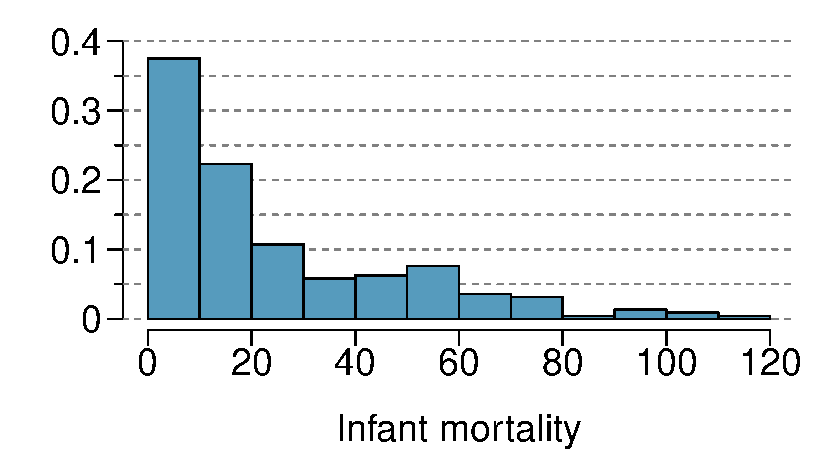
\includegraphics[width = 0.85\textwidth]{ch_summarizing_data/figures/eoce/infant_mortality_rel_freq/infant_mortality_rel_freq_hist.pdf}
\end{minipage}
}{}

% 2

\eoce{\qt{Make-up exam\label{makeup_exam}} In a class of 25 students, 24 of them took an exam 
in class and 1 student took a make-up exam the following day. The professor graded the 
first batch of 24 exams and found an average score of 74 points with a standard 
deviation of 8.9 points. The student who took the make-up the following day scored 64 
points on the exam.
\begin{parts}
\item Does the new student's score increase or decrease the average score?
\item What is the new average?
\item Does the new student's score increase or decrease the standard deviation of the 
scores?
\end{parts}
}{}

% 3

\eoce{\qt{TV watchers\label{dist_shape_TV_watchers}} Students in an AP Statistics class 
were asked how many hours of television they watch per week (including online 
streaming). This sample yielded an average of 4.71 hours, with a standard 
deviation of 4.18 hours. Is the distribution of number of hours students watch 
television weekly symmetric? If not, what shape would you expect this distribution 
to have? Explain your reasoning.
}{}

% 4

\eoce{\qt{A new statistic\label{new_stat}} The statistic $\frac{\bar{x}}{median}$ can 
be used as a measure of skewness. Suppose we have a distribution where all 
observations are greater than 0, $x_i > 0$. What is the expected shape of 
the distribution under the following conditions? Explain your reasoning.
\begin{parts}
\item $\frac{\bar{x}}{median} = 1$
\item $\frac{\bar{x}}{median} < 1$
\item $\frac{\bar{x}}{median} > 1$
\end{parts}
}{}

% 5

\eoce{\qt{Oscar winners\label{oscar_winners}} The first Oscar awards for best actor 
and best actress were given out in 1929. The histograms below show the age 
distribution for all of the best actor and best actress winners from 1929 to 
2018. Summary statistics for these distributions are also provided. Compare the 
distributions of ages of best actor and actress winners.\footfullcite{data:oscars} \\
\begin{minipage}[c]{0.72\textwidth}
\begin{center}
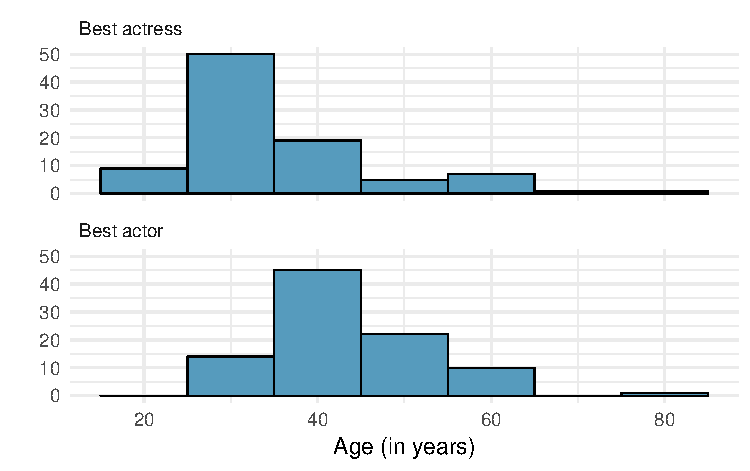
\includegraphics[width=0.95\textwidth]{ch_summarizing_data/figures/eoce/oscar_winners/oscars_winners_hist.pdf}
\end{center}
\end{minipage}
\begin{minipage}[c]{0.27\textwidth}
{\small
\begin{tabular}{l c}
\hline
        & Best Actress  \\
\hline
Mean    & 36.2      \\
SD      & 11.9      \\
n       & 92        \\  
        & \\
        & \\
        & \\
        & \\
        & \\
\hline
        & Best Actor \\
\hline
Mean    & 43.8 \\
SD      & 8.83 \\
n       & 92
\end{tabular}
}
\end{minipage}
}{}

% 6

\eoce{\qt{Exam scores\label{dist_shape_exam_scores}} The average on a history exam 
(scored out of 100 points) was 85, with a standard deviation of 15. Is the 
distribution of the scores on this exam symmetric? If not, what shape would 
you expect this distribution to have? Explain your reasoning.
}{}

% 7

\eoce{\qt{Stats scores\label{stats_scores_box}} Below are the final exam scores of twenty 
introductory statistics students.
\begin{center}
57, 66, 69, 71, 72, 73, 74, 77, 78, 78, 79, 79, 81, 81, 82, 83, 83, 88, 89, 94
\end{center}
Create a box plot of the distribution of these scores. The five number summary provided below may be useful.
\begin{center}
\renewcommand\arraystretch{1.5}
\begin{tabular}{ccccc}
Min & Q1    & Q2 (Median)   & Q3    & Max \\
\hline
57  & 72.5  & 78.5          & 82.5  & 94 \\
\end{tabular}
\end{center}
}{}

% 8

\eoce{\qt{Marathon winners\label{marathon_winners}} The histogram and box plots below show the distribution of finishing times for male and female winners of the New York Marathon between 1970 and 1999.
\begin{center}
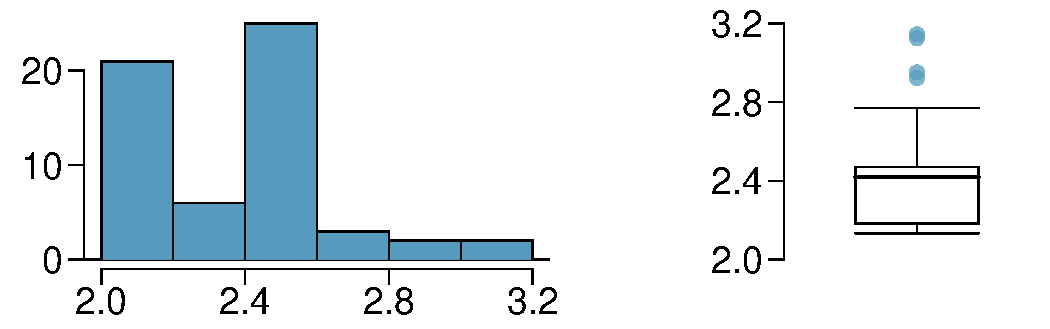
\includegraphics[width=0.56\textwidth]{ch_summarizing_data/figures/eoce/marathon_winners/marathon_winners_hist_box.pdf}
\end{center}
\begin{parts}
\item What features of the distribution are apparent in the histogram and not the box plot? What features are apparent in the box plot but not in the histogram?
\item What may be the reason for the bimodal distribution? Explain.
\item Compare the distribution of marathon times for men and women based on the box plot shown below.
\begin{center}
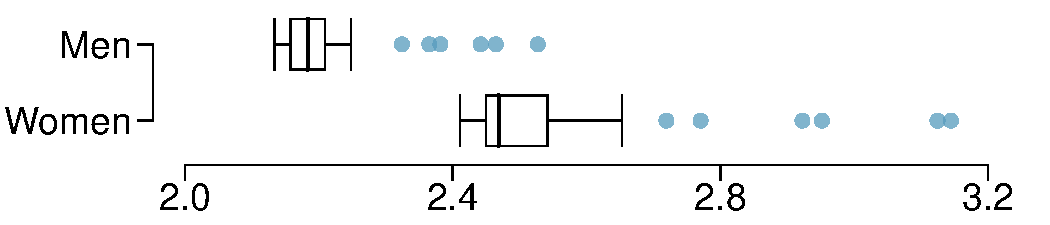
\includegraphics[width=0.56\textwidth]{ch_summarizing_data/figures/eoce/marathon_winners/marathon_winners_gender_box.pdf}
\end{center}
\item The time series plot shown below is another way to look at these data. Describe what is visible in this plot but not in the others.
\end{parts}
\begin{center}
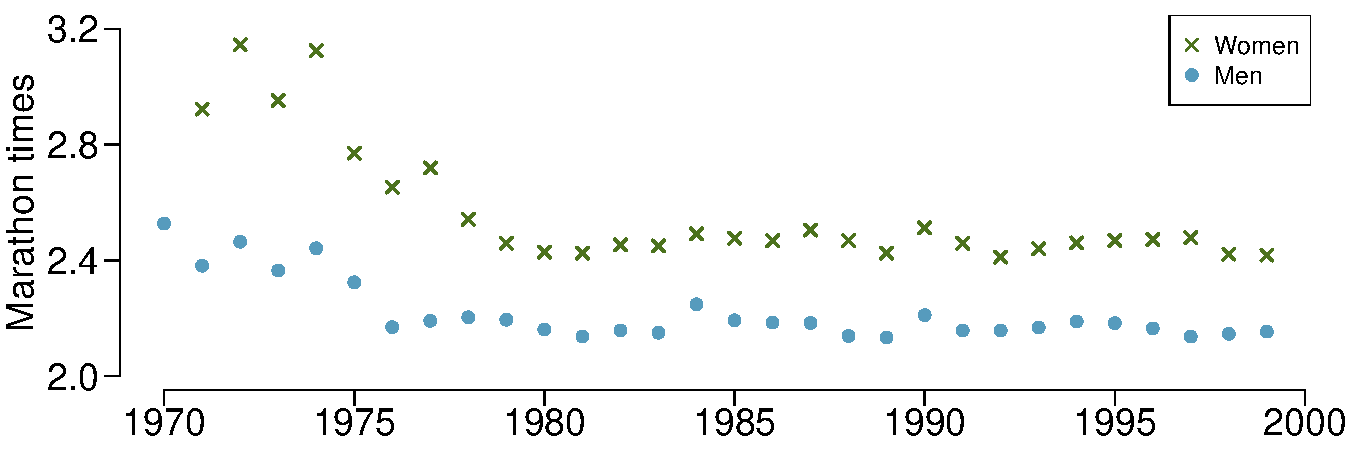
\includegraphics[width=0.6\textwidth]{ch_summarizing_data/figures/eoce/marathon_winners/marathon_winners_time_series.pdf} \\
\end{center}
}{}

  }



%-------------------------------------------------------------
% 5 Section Headers
%
% See headers.tex file for main chapters.



%-------------------------------------------------------------
% 6 Utilities
% 6.1 Helpful Editing Commands
\newcommand\Add[1]{\marginpar[{\Huge\color{oiR}$\bullet$}]{\Huge\color{oiR}$\bullet$}{\color{oiB}#1}}
\newcommand\Cut[1]{\marginpar[{\Huge\color{oiR}$\bullet$}]{\Huge\color{oiR}$\bullet$}{\color{oiGC}#1}}
%\newcommand\Comment[1]{\marginpar[{\Huge\color{oiR}$\bullet$}]{\Huge\color{oiR}$\bullet$} {\color{oiG}{[#1]}}}
\newcommand{\note}[1]{\Comment{#1}}
% 6.2 Special Symbols
\newcommand{\degree}{\ensuremath{^\circ}}
\newcommand{\R}{\textbf{\textsf{R}}}
% 6.3 Text Commands (Terms, Data, Variable, Response)
\newcommand{\term}[1]{\textbf{#1}\index{#1|textbf}}
\newcommand{\termsub}[2]{\textbf{#1}\index{#2|textbf}}
\newcommand{\termni}[1]{\textbf{#1}}
\newcommand{\hiddenterm}[1]{#1\index{#1|textbf}}
\newcommand{\indexthis}[2]{#1\index{#2}}
\newcommand{\termO}[1]{\textbf{\color{termOColor}#1}}
\newenvironment{data}[1]{\texttt{#1}}{}
\newcommand{\datalink}[1]{\index{#1|textbf}\texttt{\href{http://www.openintro.org/redirect.php?go=data_#1&referrer=\referrer}{#1}}}
\newenvironment{var}[1]{\texttt{#1}}{}
\newenvironment{resp}[1]{\texttt{#1}}{}
\newcommand{\lmlevel}[1]{:~\emph{#1}}{}
\newenvironment{calctext}[1]{{\color{oiB}\texttt{#1}}}{}
\newenvironment{calctextmath}[1]{{\color{oiB}\mathtt{#1}}}{}
\newenvironment{calcbutton}[1]{{\color{oiB}\texttt{#1}}}{}
\newcommand{\codeindent}{\hspace{5mm}}
% 6.4 Highlighting
\newenvironment{highlight}{\textbf}{}
\newcommand{\highlightO}[1]{\textbf{\color{oiB}#1}}
\newcommand{\highlightT}[1]{\emph{\color{oiR}#1}}
% 6.5 Lengths
\setlength{\parindent}{0.3in}
% 6.6 Hyperreferences
\newcommand{\urlwofont}[1]{\urlstyle{same}\url{#1}}
\newcommand{\oiRedirect}[2]{\href{http://www.openintro.org/redirect.php?go=#1&referrer=\referrer}{#2}}
\newcommand{\videoicon}[1][4.5mm]{\includegraphics[height=#1]{extraTeX/icons/video_camera.png}~}
\newcommand{\CalculatorVideos}[1]{}%{\begin{tipBox}{\tipBoxTitle[\videoicon]{Calculator videos}
%Videos covering #1 using TI and Casio graphing calculators are available at \mbox{\oiRedirect{textbook-openintro_videos}{openintro.org/videos}}.}
%\end{tipBox}}
\newcommand{\videohref}[2][4.5mm]{\oiRedirect{#2}{\raisebox{-0.3mm}[0pt]{\includegraphics[height=#1]{extraTeX/icons/video_camera.png}}}}
\newcommand{\slideshref}[2][4.5mm]{\oiRedirect{#2}{\raisebox{-0.3mm}[0pt]{\includegraphics[height=#1]{extraTeX/icons/slides.png}}}}
\newcommand{\videomarginhref}[2][4mm]{\oiRedirect{#2}{\raisebox{-3mm}[0pt]{\includegraphics[height=#1]{extraTeX/icons/video_camera.png}}}}
\newcommand{\sectionvideohref}[2][6mm]{\oiRedirect{#2}{\raisebox{-0.5mm}[0pt]{\includegraphics[height=#1]{extraTeX/icons/video_camera.png}}}}
\newcommand{\sectionslideshref}[2][6mm]{\oiRedirect{#2}{\raisebox{-0.5mm}[0pt]{\includegraphics[height=#1]{extraTeX/icons/slides.png}}}}
\newcommand{\MarginVideo}[1]{\marginpar[{\videomarginhref{#1}}]{{\videomarginhref{#1}}}}
% 6.7 Helper commands
\newcommand{\us}[0]{\_\hspace{0.3mm}}
%\newcommand{\quadplus}[0]{\quad + \quad}
\newcommand{\indfunc}[2]{\var{#1}_{\resp{#2}}}


%-------------------------------------------------------------
% 7 



%-------------------------------------------------------------
% 8 Figures and Captions
% 8.1 & 8.2 Table & Figure Numbering
% Thanks @Herbert on StackExchange for helping clean up this style code!
% http://tex.stackexchange.com/questions/176978/latex-numbering-in-counters-appears-to-have-changed/177045?noredirect=1#comment409945_177045
\makeatletter
\let\c@table\c@figure
\makeatother
% 8.3 Caption Width
\newlength{\mycaptionwidth}
\setlength{\mycaptionwidth}{0.825\textwidth}
\setlength{\captionwidth}{\mycaptionwidth}
\newcommand{\Figure}[2]{\includegraphics[width=#1\textwidth]{\chapterfolder/figures/#2/#2}}
\newcommand{\Figures}[3]{\includegraphics[width=#1\textwidth]{\chapterfolder/figures/#2/#3}}
\newcommand{\Figuress}[3]{\includegraphics[width=#1]{\chapterfolder/figures/#2/#3}}
\newcommand{\chapterfolder}{}




%-------------------------------------------------------------
% 9 Examples and Exercises
% 9.1 Exercises, within the text
% 9.1.1 Exercise Environment
\newcommand{\excolor}[1]{{\color{excolor}#1}}
\newenvironment{exercise}
{
\begin{itemize}\item[\color{oiB}$\bigodot$]\refstepcounter{equation}\noindent\normalsize\textbf{\color{oiB}Guided Practice \theexercise}%\hspace{3mm}

}
{\normalsize

\stdaddvspace{}
\end{itemize}}
% 9.1.2 Exercise Fine Tuning
\newcommand\theexercise{\thechapter.\arabic{equation}}
% 9.2 Examples
% 9.2.1 Example Environment
\newcommand\theexample{\thechapter.\arabic{equation}}
\newenvironment{example}[1]
{\begin{itemize}
\item[\color{oiB}\Large$\CIRCLE$]\refstepcounter{equation}\noindent\textbf{\color{oiB}Example \theexample}

#1\vspace{\exampleAboveBar}

{\color{examplegray}\rule{20mm}{0.1mm}}

\vspace{\exampleBelowBar}

\normalsize}{

\end{itemize}
\stdaddvspace{}
}
% 9.2.2 Wrappers
%\reversemarginpar
\def\warningsymbol{\protect\marginsymbolhelper}
\def\marginsymbolhelper{\tabto*{0mm} {\dbend} \tabto*{0mm}}
\newcommand{\exampleicon}[1]{\vspace{#1} \raggedleft
\includegraphics[width=5mm]{extraTeX/icons/example.png}\hspace{2mm}\ }
\newenvironment{gpewrapper}[1]{\addvspace{4mm}

\noindent\hspace{-12.45mm}\begin{minipage}[c]{\textwidth+8mm}
\begin{minipage}[c]{8.4mm}
\hspace{0.5mm}\includegraphics[width=5mm]{extraTeX/icons/#1.png}
\end{minipage}\begin{minipage}[c]{\textwidth-0.45mm}\begin{mdframed}[%
    topline=false,
    rightline=false,
    bottomline=false,
    linewidth=0.5mm,
    linecolor=oiB]}{\end{mdframed}\end{minipage}\end{minipage}

    \addvspace{4mm}}
\newenvironment{examplewrap}
    {\begin{gpewrapper}{example}}
    {\end{gpewrapper}}
\newenvironment{exercisewrap}
    {\begin{gpewrapper}{guided_practice}}
    {\end{gpewrapper}}
% 9.2.3 Example Title
\newcommand{\exampletitle}[1]{\textbf{\color{oiB}\small\fontfamily{phv}%
\selectfont{\MakeUppercase{Example~#1}}} \\[1mm]}
\newcommand{\exercisetitle}[1]{\textbf{\color{oiB}\small\fontfamily{phv}%
\selectfont{\MakeUppercase{Guided Practice~#1}}} \\[1mm]}
% 9.2.4 NEW Example and Guided Practice Environment
\newcommand{\exspace}{\stdvspace{}}
\newenvironment{nexample}[1]{\addvspace{6mm}

\refstepcounter{equation}\exampletitle{\theexample}
#1

\addvspace{\nexampleAboveBar}

{\color{examplegray}\rule{20mm}{0.1mm}}

\addvspace{\nexampleBelowBar}

\setlength{\parskip}{2mm}}{}
\newenvironment{nexercise}{\addvspace{6mm}

\refstepcounter{equation}\exercisetitle{\theexample}}{}

% 9.3 EOCEs: End of Chapter Exercises
% 9.3.1 Environment
\newenvironment{eoce}[2][]
{\refstepcounter{eoce}\noindent\small\textbf{\textcolor{oiB}{{\hypersetup{linkcolor=oiB}{\fontfamily{phv}\selectfont\ref{eoce_sol_\arabic{chapter}_\arabic{eoce}}}}\label{eoce_\arabic{chapter}_\arabic{eoce}}}}\hspace{2mm} #1#2

\addvspace{4mm}

}
%{\em #2 } $\:$ \\ }
{}
% 9.3.2 EOCE Solutions
\newcommand{\eocesolch}[1]{
\refstepcounter{eocesolch}\noindent\textbf{\color{oiB}\arabic{eocesolch}\hspace{2mm}#1}

\addvspace{2mm}

}
{
\newcommand{\eocesol}[1]{\refstepcounter{eocesol}\noindent\textbf{\color{oiB}{\hypersetup{linkcolor=oiB}{\fontfamily{phv}\selectfont\ref{eoce_\arabic{eocesolch}_\arabic{eocesol}}}}\label{eoce_sol_\arabic{eocesolch}_\arabic{eocesol}}}\hspace{2mm}{\small#1}\makebox[0pt]{\color{white}\tiny \refstepcounter{eocesol}\label{eoce_sol_\arabic{eocesolch}_\arabic{eocesol}}}

\addvspace{1mm}

}
% 9.3.3 EOCE Utilities
\newcommand{\qt}[2][.]{{\fontfamily{phv}\selectfont\textcolor{oiB}{\textbf{#2#1}}}}
\newcommand{\qtq}[1]{{\fontfamily{phv}\selectfont\textcolor{oiB}{\textbf{#1?}}}}
\newcommand{\ec}[1]{\textcolor{oiB}{\footnotesize{~(#1)}}}% 9.3.4 EOCE Roman Parts
\newenvironment{romanparts}{
\begin{enumerate}[I.]
\setlength{\itemsep}{0mm}
}{\end{enumerate}}
% 9.3.5 EOCE Parts
\newenvironment{parts}{
%\vspace{-0.25cm}
\begin{enumerate}[(a)]
\setlength{\itemsep}{0mm}}
{\end{enumerate}}
% 9.3.6 EOCE Subparts
\newenvironment{subparts}{
\begin{enumerate}[i.]
\setlength{\itemsep}{0mm}}
{\end{enumerate}}
% 9.3.7 EOCE hyp environment
\newenvironment{hyp}{
\begin{itemize}
\setlength{\itemsep}{0mm}
}
{\end{itemize}
}
% 9.3.8 cond environment
\newenvironment{cond}{
\begin{enumerate}[1.]
\setlength{\itemsep}{0mm}
}
{\end{enumerate}
}
% 9.3.9 Exercise fixes required.
\newcommand{\eoceNeedSolution}[1][]
{\textbf{\refstepcounter{eoceNeedSolution} \color{red}ADD SOLUTION. #1}}
\newcommand{\eoceReplace}[1][]
{\textbf{\refstepcounter{eoceReplace} \color{red}REPLACE THIS EXERCISE. #1}}
\newcommand{\eoceFF}[1][]
{\textbf{\refstepcounter{eoceFF} \color{red}FINAL FORMATTING.}}





%-------------------------------------------------------------
% 10 Special Boxes
% 10.1.1 Term Box
\newcommand\tBoxTitleBuffer{\\[1.5mm]}
\newenvironment{tBoxTitle}[2][\tBoxTitleBuffer]{\textbf{\color{oiB}#2} #1
}{}
\newenvironment{termBox}[1]{
\addvspace{4mm}
\noindent{\color{oiB}\framebox[\textwidth][c]{\framebox[\textwidth-3mm][l]{ \\
	\vspace{0.5cm} \\
	\begin{minipage}[b]{\textwidth-3mm}
		\begin{minipage}[t]{2mm}
			\hspace{2mm}
		\end{minipage}
		\begin{minipage}[b]{\textwidth-10mm}
			\color{black}\ \\[-0.7mm]
			#1
			
			\vspace{1mm}
		\end{minipage}
	\end{minipage}}}}
}{

\addvspace{1mm}}
% 10.2 Tip Box
\newenvironment{tipBoxTitle}[2][TIP:\ ]{\textbf{\color{oiB}#1#2}\\[0.3mm]}{}
\newenvironment{tipBox}[1]{
\addvspace{4mm}
\noindent{\color{oiB}\framebox[\textwidth][l]{ \\
	\vspace{5mm} \\
	\begin{minipage}[b]{\textwidth-4mm}
		\begin{minipage}[t]{2mm}
			\hspace{2mm}
		\end{minipage}
		\begin{minipage}[b]{\textwidth-8mm}
			\color{black}\ \\[-0.7mm]
			#1
			
			\vspace{1mm}
		\end{minipage}
	\end{minipage}}}
}{

\addvspace{1mm}}
% 10.3 Caution Box
\newenvironment{caution}[2]{
\addvspace{4mm}
\noindent{\color{oiB}\framebox[\textwidth][l]{ \\
	\vspace{5mm} \\
	\begin{minipage}[b]{\textwidth-4mm}
		\begin{minipage}[t]{2mm}
			\hspace{2mm}
		\end{minipage}
		\begin{minipage}[b]{\textwidth-8mm}
			\textbf{\color{oiB}Caution: #1} \\[1mm]
			\color{black}#2
		\end{minipage}
	\end{minipage}}}
}{

\addvspace{1mm}}
% 10.4 One Box
\newenvironment{onebox}[1]{
\addvspace{4mm}
\noindent\begin{minipage}{\textwidth}
\noindent\rule{\textwidth}{0.3pt}\vspace{-6mm}
\begin{mdframed}[%
    topline=false,
    rightline=false,
    leftline=false,
    bottomline=false,
    backgroundcolor=grayBackground]
\textbf{\color{oiB}\small\fontfamily{phv}%
\selectfont{\MakeUppercase{#1}}} \\[1mm]}{
\end{mdframed}\vspace{-4.2mm}
\rule{\textwidth}{0.3pt}
\end{minipage}

\addvspace{4mm}}



